% Options for packages loaded elsewhere
% Options for packages loaded elsewhere
\PassOptionsToPackage{unicode,linktoc=all}{hyperref}
\PassOptionsToPackage{hyphens}{url}
\PassOptionsToPackage{dvipsnames,svgnames,x11names}{xcolor}
%
\documentclass[
  letterpaper,
  DIV=11,
  numbers=noendperiod]{scrreprt}
\usepackage{xcolor}
\usepackage[top=30mm,left=20mm,heightrounded]{geometry}
\usepackage{amsmath,amssymb}
\setcounter{secnumdepth}{5}
\usepackage{iftex}
\ifPDFTeX
  \usepackage[T1]{fontenc}
  \usepackage[utf8]{inputenc}
  \usepackage{textcomp} % provide euro and other symbols
\else % if luatex or xetex
  \usepackage{unicode-math} % this also loads fontspec
  \defaultfontfeatures{Scale=MatchLowercase}
  \defaultfontfeatures[\rmfamily]{Ligatures=TeX,Scale=1}
\fi
\usepackage{lmodern}
\ifPDFTeX\else
  % xetex/luatex font selection
  \setmainfont[]{Calibri}
\fi
% Use upquote if available, for straight quotes in verbatim environments
\IfFileExists{upquote.sty}{\usepackage{upquote}}{}
\IfFileExists{microtype.sty}{% use microtype if available
  \usepackage[]{microtype}
  \UseMicrotypeSet[protrusion]{basicmath} % disable protrusion for tt fonts
}{}
\makeatletter
\@ifundefined{KOMAClassName}{% if non-KOMA class
  \IfFileExists{parskip.sty}{%
    \usepackage{parskip}
  }{% else
    \setlength{\parindent}{0pt}
    \setlength{\parskip}{6pt plus 2pt minus 1pt}}
}{% if KOMA class
  \KOMAoptions{parskip=half}}
\makeatother
% Make \paragraph and \subparagraph free-standing
\makeatletter
\ifx\paragraph\undefined\else
  \let\oldparagraph\paragraph
  \renewcommand{\paragraph}{
    \@ifstar
      \xxxParagraphStar
      \xxxParagraphNoStar
  }
  \newcommand{\xxxParagraphStar}[1]{\oldparagraph*{#1}\mbox{}}
  \newcommand{\xxxParagraphNoStar}[1]{\oldparagraph{#1}\mbox{}}
\fi
\ifx\subparagraph\undefined\else
  \let\oldsubparagraph\subparagraph
  \renewcommand{\subparagraph}{
    \@ifstar
      \xxxSubParagraphStar
      \xxxSubParagraphNoStar
  }
  \newcommand{\xxxSubParagraphStar}[1]{\oldsubparagraph*{#1}\mbox{}}
  \newcommand{\xxxSubParagraphNoStar}[1]{\oldsubparagraph{#1}\mbox{}}
\fi
\makeatother


\usepackage{longtable,booktabs,array}
\newcounter{none} % for unnumbered tables
\usepackage{calc} % for calculating minipage widths
% Correct order of tables after \paragraph or \subparagraph
\usepackage{etoolbox}
\makeatletter
\patchcmd\longtable{\par}{\if@noskipsec\mbox{}\fi\par}{}{}
\makeatother
% Allow footnotes in longtable head/foot
\IfFileExists{footnotehyper.sty}{\usepackage{footnotehyper}}{\usepackage{footnote}}
\makesavenoteenv{longtable}
\usepackage{graphicx}
\makeatletter
\newsavebox\pandoc@box
\newcommand*\pandocbounded[1]{% scales image to fit in text height/width
  \sbox\pandoc@box{#1}%
  \Gscale@div\@tempa{\textheight}{\dimexpr\ht\pandoc@box+\dp\pandoc@box\relax}%
  \Gscale@div\@tempb{\linewidth}{\wd\pandoc@box}%
  \ifdim\@tempb\p@<\@tempa\p@\let\@tempa\@tempb\fi% select the smaller of both
  \ifdim\@tempa\p@<\p@\scalebox{\@tempa}{\usebox\pandoc@box}%
  \else\usebox{\pandoc@box}%
  \fi%
}
% Set default figure placement to htbp
\def\fps@figure{htbp}
\makeatother





\setlength{\emergencystretch}{3em} % prevent overfull lines

\providecommand{\tightlist}{%
  \setlength{\itemsep}{0pt}\setlength{\parskip}{0pt}}



 


\usepackage{circuitikz}
\usetikzlibrary{arrows.meta}
\KOMAoption{captions}{tableheading}
\makeatletter
\@ifpackageloaded{caption}{}{\usepackage{caption}}
\AtBeginDocument{%
\ifdefined\contentsname
  \renewcommand*\contentsname{Table of contents}
\else
  \newcommand\contentsname{Table of contents}
\fi
\ifdefined\listfigurename
  \renewcommand*\listfigurename{List of Figures}
\else
  \newcommand\listfigurename{List of Figures}
\fi
\ifdefined\listtablename
  \renewcommand*\listtablename{List of Tables}
\else
  \newcommand\listtablename{List of Tables}
\fi
\ifdefined\figurename
  \renewcommand*\figurename{Figure}
\else
  \newcommand\figurename{Figure}
\fi
\ifdefined\tablename
  \renewcommand*\tablename{Table}
\else
  \newcommand\tablename{Table}
\fi
}
\@ifpackageloaded{float}{}{\usepackage{float}}
\floatstyle{ruled}
\@ifundefined{c@chapter}{\newfloat{codelisting}{h}{lop}}{\newfloat{codelisting}{h}{lop}[chapter]}
\floatname{codelisting}{Listing}
\newcommand*\listoflistings{\listof{codelisting}{List of Listings}}
\makeatother
\makeatletter
\makeatother
\makeatletter
\@ifpackageloaded{caption}{}{\usepackage{caption}}
\@ifpackageloaded{subcaption}{}{\usepackage{subcaption}}
\makeatother
\usepackage{bookmark}
\IfFileExists{xurl.sty}{\usepackage{xurl}}{} % add URL line breaks if available
\urlstyle{same}
\hypersetup{
  pdftitle={VCO Design und Simulation},
  pdfauthor={Mirco Ick; Torben Becker; Tassilo Hertling},
  colorlinks=true,
  linkcolor={blue},
  filecolor={Maroon},
  citecolor={Blue},
  urlcolor={Blue},
  pdfcreator={LaTeX via pandoc}}


\title{VCO Design und Simulation}
\author{Mirco Ick \and Torben Becker \and Tassilo Hertling}
\date{2026-05-08}
\begin{document}
\maketitle

\renewcommand*\contentsname{Table of contents}
{
\setcounter{tocdepth}{2}
\tableofcontents
}

\chapter{Introduction}\label{introduction}

In diesesm Projekt gilt es einen VCO (Voltage Controlled Oszillator) zu
designen und in Betrieb zu nehmen. Das Design soll bestimmte
Anforderungen erfüllen, damit es in einem Laborversuch als FM-Modulator
genutzt werden kann. In der Vergangenheit wurde im Laborversuch eine VCO
Schaltung mit alten und abgekündigkten Komponenten verwendet. Diese
Schaltung soll nun mit neuen und verfügbaren Komponenten erneuert
werden.

Die VCO Schaltung soll eine FM-Modulation mit einem Trägersignal bei der
Frequenz \(5,5\,\text{MHz}\) durchführen und einen Modulationsbereich
zwischen \(5\,\text{MHz}\) und \(6\,\text{MHz}\) verwenden. Der
Einstellungsbereich soll mit \(1\,\text{V}\) pro \(1\,\text{MHz}\)
eingestellt werden. Somit kann das zu modulierende Signal einen
Spannungsbereich von \(V_{pp} = 1\,\text{V}\) haben. Die Ein- und
Ausgangsimpedanz soll \(50\,\Omega\) betragen.

Zudem soll die Schaltung soll aus Komponenten bestehen, die Studierenden
im 4.Semester bereits kennen, damit die Schaltung im Rahmen des
Laborversuchs im Grunde verstanden werden kann. Aus dieser
Rahmenbedingung folgt die Auswahl der spezifischen VCO-Schaltung.

Die Platine soll zudem relativ groß ausgelegt werden und es sollen
möglichst bedrahtete Bauteile verwendet werden. In dem Laborversuch soll
ebenfalls die Kennlinie des FM-Modulators aufgenommen werden. Hierfür
ist ein integrierter einstellbarer Spannungsteiler vorgesehen, der über
einen Drehregler auf der Platine eingestellt werden soll.

Die Schaltung soll ebenfalls Stabil gegenüber Schwankungen in der
Versorgungsspannung und somit in der Ausgangsfrequenz ausgelegt sein.
Anschlüsse für die im Laborversuch verwendeten Geräte wie das
Oszilloskop und dem Spektrumanalysator sollen über SMA- oder
BNC-Anschlüsse geschehen.

\chapter{Designverlauf}\label{designverlauf}

Zuerst haben wir im Design angefangen uns ein passendes VCO-Modell nach
den Anforderungen auszusuchen. Als Modell haben wir uns für den LC-VCO
entschieden. Dieser besteht im Grunde aus einer RLC-Schaltung und einer
kreuzgekoppelten Mosfet-Schaltung. Das Design ist somit gut für
Studierende aus dem 4. Semester zu verstehen und kann auch gut mit
bedrahteten Bauteilen aufgebaut werden. Die Grundschaltung ist in
Abbildung 1 zu sehen:

\begin{figure}[H]

{\centering 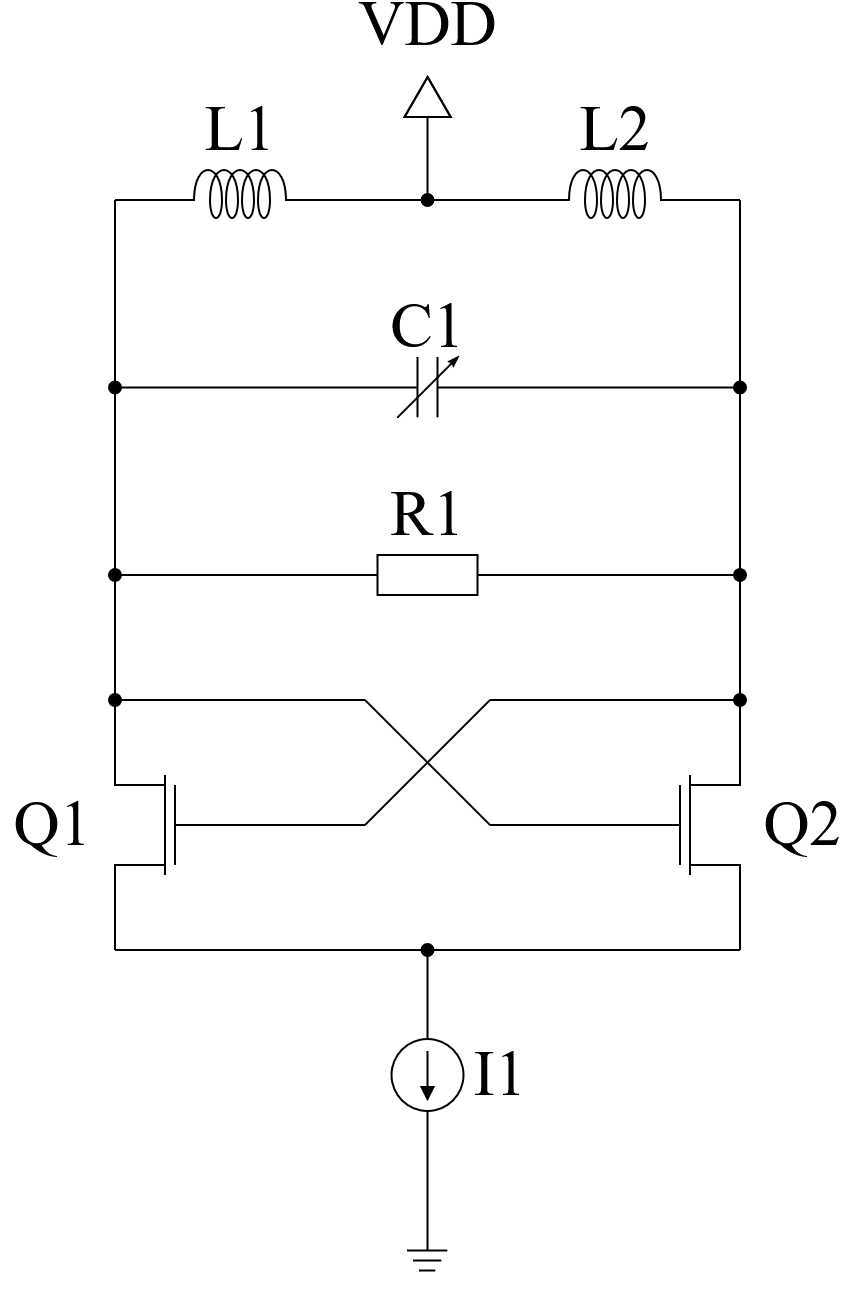
\includegraphics[width=0.6\linewidth,height=\textheight,keepaspectratio]{./images/circuit.png}

}

\caption{Bild1}

\end{figure}%

\chapter{Characterisation}\label{characterisation}

\chapter*{Literaturverzeichnis}\label{literaturverzeichnis}
\addcontentsline{toc}{chapter}{Literaturverzeichnis}

\protect\phantomsection\label{refs}




\end{document}
